\documentclass[tikz,border=10pt]{standalone}
\usetikzlibrary{calc}
\begin{document}
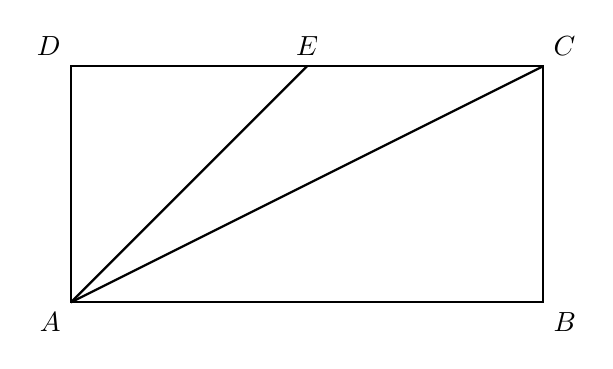
\begin{tikzpicture}[scale=2, thick]    
% 定义基础坐标，比例约为 2:1    
\coordinate (A) at (0,0);    
\coordinate (B) at (3,0);    
\coordinate (C) at (3,1.5);    
\coordinate (D) at (0,1.5);        
% 定义点 E，根据图片比例，E 大约在 CD 的三分之二处    
\coordinate (E) at (1.5,1.5);         
% 绘制矩形边界    
\draw (A) -- (B) -- (C) -- (D) -- cycle;        
% 绘制辅助线 AE 和 AC    
\draw (A) -- (E);    
\draw (A) -- (C);        
% 标注顶点    
\node[below left]  at (A) {$A$};    
\node[below right] at (B) {$B$};    
\node[above right] at (C) {$C$};    
\node[above left]  at (D) {$D$};    
\node[above]       at (E) {$E$};    
\end{tikzpicture}
\end{document}